\documentclass[12pt]{article}
\usepackage[T1,T2A]{fontenc}
\usepackage[utf8]{inputenc}
\usepackage{graphicx}
\usepackage[english, russian]{babel}
\usepackage[colorlinks=true, 
linkcolor=blue,
filecolor=blue,
citecolor=blue, 
urlcolor=blue,
unicode=true]{hyperref} %для ссылок
\usepackage{graphicx} % для фотографии
\usepackage{mathtools}
\usepackage{amsmath,amssymb,amsthm,latexsym}
\usepackage{mathtext}
\usepackage{multirow}
\usepackage{indentfirst}
\usepackage{enumerate}
\usepackage{verbatim}
\usepackage{multirow}
\usepackage{bigstrut}
\usepackage{booktabs}
\usepackage[left=12mm, top=10mm, right=15mm, bottom=15mm, nohead, footskip=10mm]{geometry} % настройки полей документа
\usepackage{wrapfig}
\usepackage{array}
\usepackage[rightcaption]{sidecap} % для подписей справа
\usepackage{color,colortbl}

\definecolor{darkishgreen}{RGB}{39,203,22}
\definecolor{LightCyan}{rgb}{0.88,1,1}
\definecolor{Gray}{gray}{0.8}
\definecolor{lightRed}{RGB}{230,170,150}
\definecolor{modRed}{RGB}{230,82,90}
\definecolor{strongRed}{RGB}{230,6,6}

\author{Барсуков Максим}
\title{Рабочий протокол и отчет по лабораторной работе № \\}
\date{\today}

\begin{document}

\begin{table}[htbp]
	\centering
	\begin{tabular}{lrlr}
		Группа & \qquad \qquad P3215 & К работе допущен & \qquad \qquad \qquad \qquad \qquad \qquad \\
		\cmidrule{2-2}\cmidrule{4-4}         
		Студент &  \qquad \qquad Барсуков М.А.  & Работа выполнена & \qquad \qquad \qquad \qquad \qquad \qquad \\
		\cmidrule{2-2}\cmidrule{4-4}          
		Преподаватель & \qquad \qquad Смирнов А.В. & Отчет принят & \qquad \qquad \qquad \qquad \qquad \qquad \\
		\cmidrule{2-2}\cmidrule{4-4}    
	\end{tabular}%
\end{table}%

\begin{center}
    \huge\textbf{Рабочий протокол и отчет\\по лабораторной работе №3.03}\\"Определение удельного заряда электрона"
\end{center}

\section{Цель работы}
Определить удельный заряд электрона методом магнетрона.

\section{Задачи, решаемые при выполнении работы}
\begin{itemize}
\item 1. Провести измерения зависимости анодного тока $I_a$ вакуумного
диода от величины тока в соленоиде при различных значениях анодного напряжения.
\item 2. Построить графики зависимостей $I_a$ от B и определить по ним величины критических полей для каждого значения анодного напряжения.
\item 3. По значениям критического поля найти величину удельного заряда электрона и оценить ее погрешность.
\end{itemize}

\section{Объект исследования}
Анодный ток в соосном вакуумном диоде под действием магнитного поля соленойдной обмотки.

\section{Метод экспериментального исследования}
Измерение анодного тока при изменении тока на соленоиде при различном напряжении на аноде.

\section{Рабочие формулы и исходные данные}

Радиус анода: $r_a = 3$ \textit{мм}

Диаметр катушки: $d=37$ \textit{мм}

Длина катушки: $l=36$ \textit{мм}

Число витков катушки: $N=1500$ \\

Удельный заряд электрона:
\begin{equation}
    \frac{e}{m}=\frac{8U}{B_c^2r_a^2}
    \label{eqn:specific_charge}
\end{equation} \\
где $U$ - анодное напряжение, $r=r_a$ и $B=B_c$ - критическое значение магнитной индукции (только в таком случае траектория электронов будет касательной к аноду): \\

Магнитное поле внутри соленоида конечной длины в СИ ($\mu_0\cong1,256637\cdot10^{-6} \frac{\textit{Н}}{\textit{А}^{2}}$):
\begin{equation}
     B=\frac{\mu_0 IN}{\sqrt{d^2+l^2}}
     \label{eqn:critic_induction}
\end{equation}

\section{Измерительные приборы}
\begin{center}
\begin{tabular}{ | m{0.5cm} | m{7cm}| m{3cm} | m{3cm} | m{3cm} | } 
  \hline
  № & Наименование & Тип прибора & Используемый диапазон & Погрешность прибора \\ 
  \hline
  1 & Мультиметр в режиме амперметра & электронный& $0\div 10$ \textit{А}& 0,005 \textit{А} \\ 
  \hline
   2 & Мультиметр в режиме амперметра &электронный & $0 \div 2 $ \textit{мА}& 0,05 \textit{мкА}\\ 
   \hline
   3 & Вольтметр & электронный & $9\div13$ \textit{В}& 0,05 \textit{В}\\
  \hline
\end{tabular}
\end{center}

\section{Схема установки}
\begin{SCfigure}[0.5][h!]
\caption{Принципиальная электрическая схема экспериментальной установки}
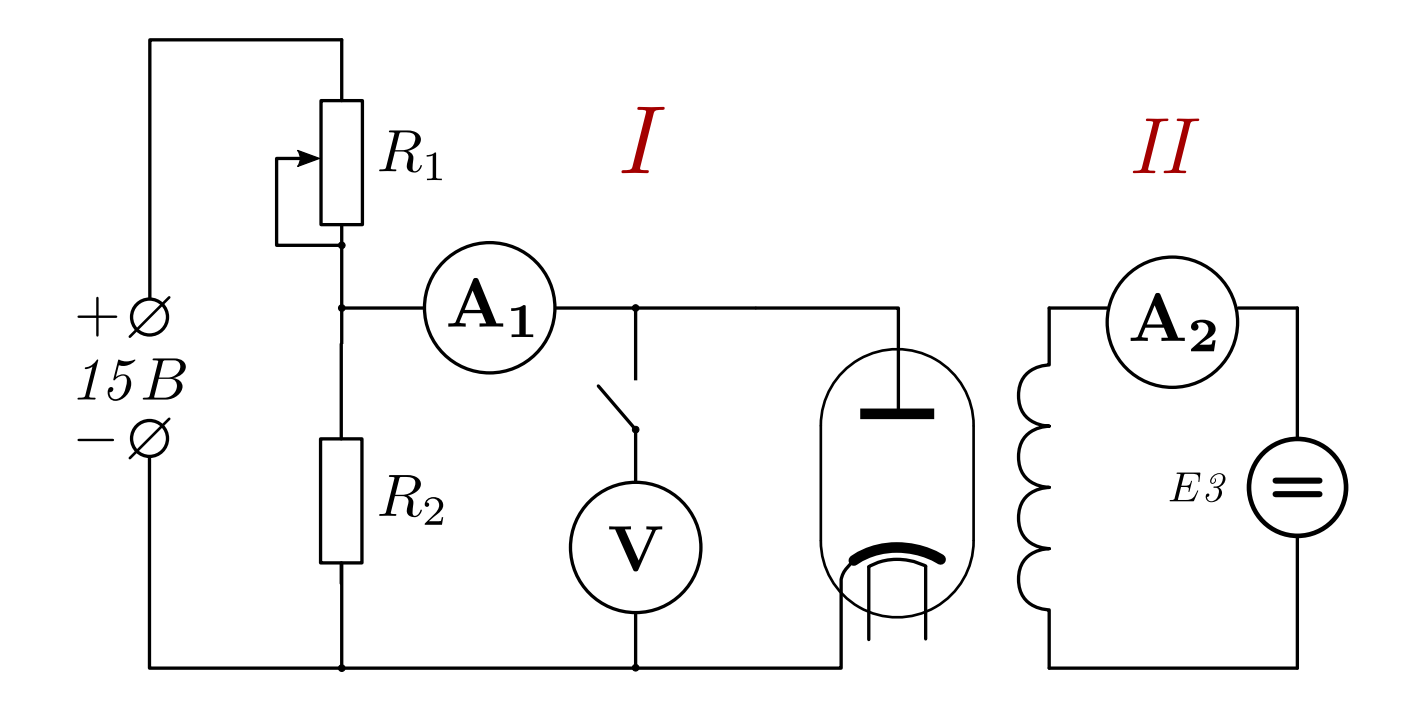
\includegraphics[width=0.7\textwidth]{scheme.png}
\end{SCfigure}

\newpage

\section{Результаты прямых измерений и их обработки}
\newcolumntype{g}{>{\columncolor{Gray}}c}
\newcolumntype{d}{>{\columncolor{darkishgreen}}c}
\begin{table}[h!]
    \centering
    \begin{tabular}{|l|l|l|l|l|l|}
    \hline
        № опыта & i & \multicolumn{2}{l|}{1} & \multicolumn{2}{l|}{3} \\ \hline
        ~ & $U_{ai}$, $\textit{В}$ & \multicolumn{2}{l|}{9} & \multicolumn{2}{l|}{13,5}  \\ \hline
        $I_c$, $\textit{А}$ & B, $\textit{мТл}$ & $I_{a1}$, \textit{мкA} & $\Delta{I_{a1}}/\Delta{B}$ & $I_{a3}$, $\textit{мкА}$ & $\Delta{I_{a3}}/\Delta{B}$  \\ \hline
        0,00 & 0,00 & 222,0 & ~ & 359,2 & ~ \\ \hline
        0,02 & 0,73 & 222,0 & 0,00 & 359,3 & 0,14 \\ \hline
        0,04 & 1,46 & 221,8 & -0,27 & 359,4 & 0,14 \\ \hline
        0,06 & 2,19 & 222,1 & 0,41 & 359,5 & 0,14 \\ \hline
        0,08 & 2,92 & 222,0 & -0,14 & 359,6 & 0,14 \\ \hline
        0,10 & 3,65 & 222,0 & 0,00 & 359,7 & 0,14 \\ \hline
        0,12 & 4,38 & 222,3 & 0,41 & 360,2 & 0,68 \\ \hline
        0,14 & 5,11 & 222,1 & -0,27 & 361,7 & 2,05 \\ \hline
        0,16 & 5,84 & 221,1 & -1,37 & 362,2 & 0,68 \\ \hline
        0,18 & 6,57 & 218,6 & -3,42 & 361,1 & -1,51 \\ \hline
        0,20 & 7,30 & 211,9 & -9,18 & 356,4 & -6,44 \\ \hline
        \cellcolor{Gray} 0,22 & 8,03 & 199,7 & -16,71 & 348,7 & -10,55 \\ \hline
        \cellcolor{Gray} 0,24 & 8,76 & 144,0 & \cellcolor{Gray} -76,30 & 304,4 & -60,68 \\ \hline
        \cellcolor{Gray} 0,26 & 9,49 & 124,3 & -26,99 & 222,8 & \cellcolor{Gray} -111,78 \\ \hline
        0,28 & 10,22 & 104,5 & -27,12 & 198,7 & -33,01 \\ \hline
        0,30 & 10,95 & 88,9 & -21,37 & 166,8 & -43,70 \\ \hline
        0,32 & 11,68 & 75,6 & -18,22 & 153,0 & -18,90 \\ \hline
        0,34 & 12,41 & 66,1 & -13,01 & 140,5 & -17,12 \\ \hline
        0,36 & 13,14 & 58,9 & -9,86 & 125,6 & -20,41 \\ \hline
        0,38 & 13,88 & 51,3 & -10,27 & 116,1 & -12,84 \\ \hline
        0,40 & 14,61 & 47,4 & -5,34 & 104,6 & -15,75 \\ \hline
        0,42 & 15,34 & 42,5 & -6,71 & 96,9 & -10,55 \\ \hline
        0,44 & 16,07 & 39,5 & -4,11 & 87,6 & -12,74 \\ \hline
        0,46 & 16,80 & 35,4 & -5,62 & 80,8 & -9,32 \\ \hline
        0,48 & 17,53 & 34,1 & -1,78 & 74,2 & -9,04 \\ \hline
        0,50 & 18,26 & 31,0 & -4,25 & 69,0 & -7,12 \\ \hline
    \end{tabular}
    \caption{Результаты прямых измерений токов на аноде и на соленоиде и дальнейших расчетов (в выделенных ячейках - значения максимального отношения изменения анодного тока к изменению магнитного поля и соответственные им значения тока на соленойде)}
\end{table}

\section{Расчет результатов косвенных измерений}
По формуле (2) были рассчитаны значения B для каждого тока на соленойдной обмотке, данные внесены в Таблицу 1.
Зависимости анодного тока от магнитного поля соленойда представлены на Рис.2

Для каждого из значений анодного напряжения было найдено отношение изменения тока на аноде к изменению магнитного поля. При максимальном значении $|\frac{\Delta I_a}{\Delta I_c}|$ будет наблюдаться скорейшее изменение $I_a$, а значит и $B$, связанного с ним. Таким образом найдены критические значения силы тока на соленойде $I_\text{кр}$ = $\frac{I_{c2}+I_{c1}}{2}$ - то есть взято среднее значение тока на отрезке, удовлетворяющему максимальному изменению $\Delta{B}$. Для каждого из анодных напряжений и значений критических токов по формуле \ref{eqn:critic_induction} было рассчитано критическое значение магнитной индукции:\\ \\
$U=9\text{ В}: I_{\text{кр}}=0,23 \textit{ А, }B_c=8,4\textit{ мТл}\\
U=13,5\text{ В}:  I_{\text{кр}}=0,25 \textit{ А, }B_c=9,13\textit{ мТл}$\\

Удельный заряд электронов для каждого из значений анодного напряжении и критического значения силы тока рассчитывался по формуле \ref{eqn:specific_charge}:\\ \\
$U=9\text{ В}: \frac{e}{m}=1,134\cdot10^{11} \textit{ Кл/кг}\\
U=13,5\text{ В}: \frac{e}{m}=1,44\cdot10^{11} \textit{ Кл/кг}$\\

Среднее значение удельного заряда электрона (полученное с помощью метода весов):
$$\langle \frac{e}{m} \rangle = 1,25\cdot10^{11} \textit{ Кл/кг} $$

\section{Расчет погрешностей измерений}
Примем значения погрешностей: \\
$\Delta{r} = 0,05 \textit{мм}$ \\
$\Delta{d} = 0,5 \textit{мм}$ \\ 
$\Delta{l} = 0,5 \textit{мм}$ \\
$\Delta{I_{kp}} = 0,02 \textit{А}$ - так как $B \sim I_c$ $\Rightarrow$ графическая погрешность определения критического значения = 0,01 \textit{А}; приборная погрешность = $\frac{\Delta I_{c1}+ \Delta I_{c2}}{2} \approx 0,005 \textit{А}$ \\

Оценим погрешность удельного заряда электрона:
\begin{equation*}
    \Delta \frac{e}{m}=\frac{e}{m}\sqrt{\bigg(\frac{\Delta U}{U}\bigg)^2+\bigg(2\frac{\Delta r}{r}\bigg)^2+\bigg(2\frac{\Delta I_{\text{кр}}}{I_{\text{кр}}}\bigg)^2+\bigg(2\frac{\Delta l}{l}\bigg)^2+\bigg(2\frac{\Delta d}{d}\bigg)^2}
\end{equation*} \\

Вычислим для каждого из значений анодного напряжения и критического тока:
\begin{equation*}
    \bigg(\Delta \frac{e}{m}\bigg)_1=1,134\cdot10^{11}\sqrt{\bigg(\frac{0,05}{9}\bigg)^2+\bigg(\frac{0,05}{3}\bigg)^2+\bigg(2\frac{0,015}{0,23}\bigg)^2+\bigg(2\frac{0,5}{37}\bigg)^2+\bigg(2\frac{0,5}{36}\bigg)^2} \approx 0,15\cdot10^{11}\textit{ Кл/кг}
\end{equation*}
\begin{equation*}
    \bigg(\Delta \frac{e}{m}\bigg)_3 \approx 0,19\cdot10^{11}\textit{ Кл/кг}
\end{equation*} \\

Погрешность среднего значения (вычесленная по методу весов):
\begin{equation*}
    \Delta \langle \frac{e}{m} \rangle \approx 0,12\cdot10^{11} \textit{ Кл/кг}
\end{equation*}

\newpage
\section{Графики}
\begin{figure}[h!]
    \centering
    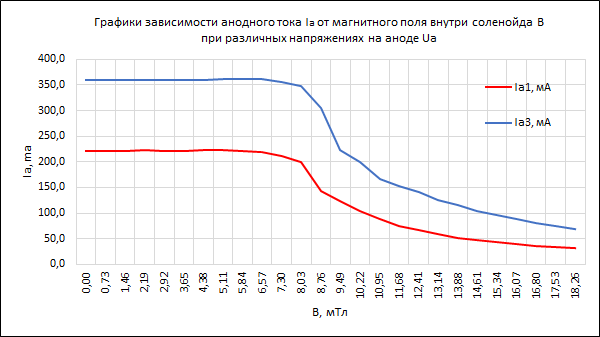
\includegraphics[width = 1\textwidth]{3.03.png}
    \begin{flushright}   
    Рис.2
    \end{flushright}
\end{figure}

\section{Окончательные результаты}

Среднее значение удельного заряда электрона:
$$\frac{e}{m} = (1,25\pm0,12)\cdot10^{11} \textit{ Кл/кг} $$

Табличное значение удельного заряда электрона:
$$\frac{e}{m} \cong 1,76\cdot10^{11} \textit{ Кл/кг} $$

\newpage
\section{Выводы и анализ результатов работы}
В ходе работы был определен удельный заряд электрона методом магнетрона. При сравнении экспериментального значения с табличным заметно, что табличное значение не попадает в доверительный интервал. Такое расхождение возможно обусловлено упомянутым в методических указаниях влиянием облака заряда, накапливающегося в диоде. Заметно, что с увеличением напряжения на аноде растет и удельный заряд электрона, приближаясь к  табличному значению. Следовательно, при больших значениях анодного напряжения влияние накапливающихся в диоде облака электронов уменьшается.

\end{document}
